\documentclass{article} % For LaTeX2e
\usepackage{nips13submit_e,times}
\usepackage{hyperref}
\usepackage{url}
\usepackage{graphicx}
%\documentstyle[nips13submit_09,times,art10]{article} % For LaTeX 2.09


\title{Formatting Instructions for NIPS 2013}


\author{
Jonathan Yee\\
\texttt{jyee1@andrew.cmu.edu} \\
\And
Lingzhang Jiang \\
\texttt{lingzhaj@andrew.cmu.edu} \\
}

% The \author macro works with any number of authors. There are two commands
% used to separate the names and addresses of multiple authors: \And and \AND.
%
% Using \And between authors leaves it to \LaTeX{} to determine where to break
% the lines. Using \AND forces a linebreak at that point. So, if \LaTeX{}
% puts 3 of 4 authors names on the first line, and the last on the second
% line, try using \AND instead of \And before the third author name.

\newcommand{\fix}{\marginpar{FIX}}
\newcommand{\new}{\marginpar{NEW}}

\nipsfinalcopy % Uncomment for camera-ready version

\begin{document}


\maketitle

\begin{abstract}
I dunno what to put here lol
\end{abstract}

\section{Background}
We are trying to apply different machine learning techniques to an Optical Character Recognition(OCR) problem, with the objective of obtaining a high level of accuracy comparable on a given data-set comparable to state-of-the-art techniques.

OCR can be analyzed using the noisy channel model, with the source being the human mind, and the channel being the handwriting technique. We want to determine the most likely letter given the handwriting. 

For this project, we intend to design a Hidden Markov Model. The hidden states of the HMM will be the letters the human is thinking of, and the observed output is the actual handwriting represented as a pixel vector. This HMM can be graphically represented as a Bayes net. The goal is to find the sequence of hidden states (i.e. letters) that maximize the joint probability of those characters and the pixel vectors. Various OCR techniques (neural networks, naive bayes, logistic regression) can be applied to determine the probabilities that a pixel vector is a certain letter. We also intend to use the Viterbi algorithm to determine the most likely sequence of letters.

\section{Related Work}
The first related work we looked at was a similar study by Ivan Dervisevic[1], which utilized four classifiers(Naive Bayes, Complement Naive Bayes, SMO, and C4.5) to perform OCR and compared the results of these classifiers. SMO is a kind of support vector machine classifier while C4.5 is a decision tree classifier. The dataset that was used contained capital characters from 238 TrueType fonts and the data was 40x40 pixel images of each character. In addition to using the raw unprocessed pixel image data, refined datasets with processed representations of the characters were also used. As our focus is more on the machine learning portion and less on the image processing techniques, we will only be using 2 classifiers as a baseline, leaving out image processing, and focusing on implementing a HMM to optimize classification instead.


\section{Methods}
To obtain our baselines, we picked two machine learning learning methods that were taught in class, Naive Bayes and Logistic Regression. Both of these methods would take as inputs a data array containing the pixel data of a collection of handwritten characters as well as a vector containing the labels for the data array. After training the classifiers on the training set, we ran the trained classifiers on a test data set for which we know the correct labels, and compared the predicted labels with the correct labels to get the accuracy of the classifiers. Also, we did cross-validation to get a confident accuracy rating for our baseline methods. 

\section{Experiments}
Description of data set

\section{Results}
\subsection{Naive Bayes}
For our first baseline we performed Naive Bayes on the raw pixel data.
If given some character $c$ and an array of n binary pixel values $\{p_1, ..., p_n\}$, the algorithm is based on basic Bayes rule:
$$P(c|p_1, p_2, ... , p_n) = \frac{P(p_1, p_2, ... , p_n|c)p(c)}{p(p_1, p_2, ... , p_n)}$$
If we make the assumptions that individual pixels are conditionally independent given some character then we can expand the conditional probability in the numerator. Using the naive bayes algorithm in the statistics toolbox for Matlab, we ran Naive Bayes over our dataset consisting of pixel data for 52152 characters(26 unique characters, no capitals) with each observation having 128 binary pixel values.

N-fold cross validation splits the data into N disjoint sets. In each of N iterations training is done on N-1 sets and testing is done on the remaining 1 set. If we take the mean accuracy we can then average out errors resulting from variance.

We performed 10-fold cross validation for our Naive Bayes classifier and were able to obtain a final accuracy of 62.7\%.

\subsection{Logistic Regression}

\subsection{Baseline Comparison}
\begin{figure}[h]
\begin{center}
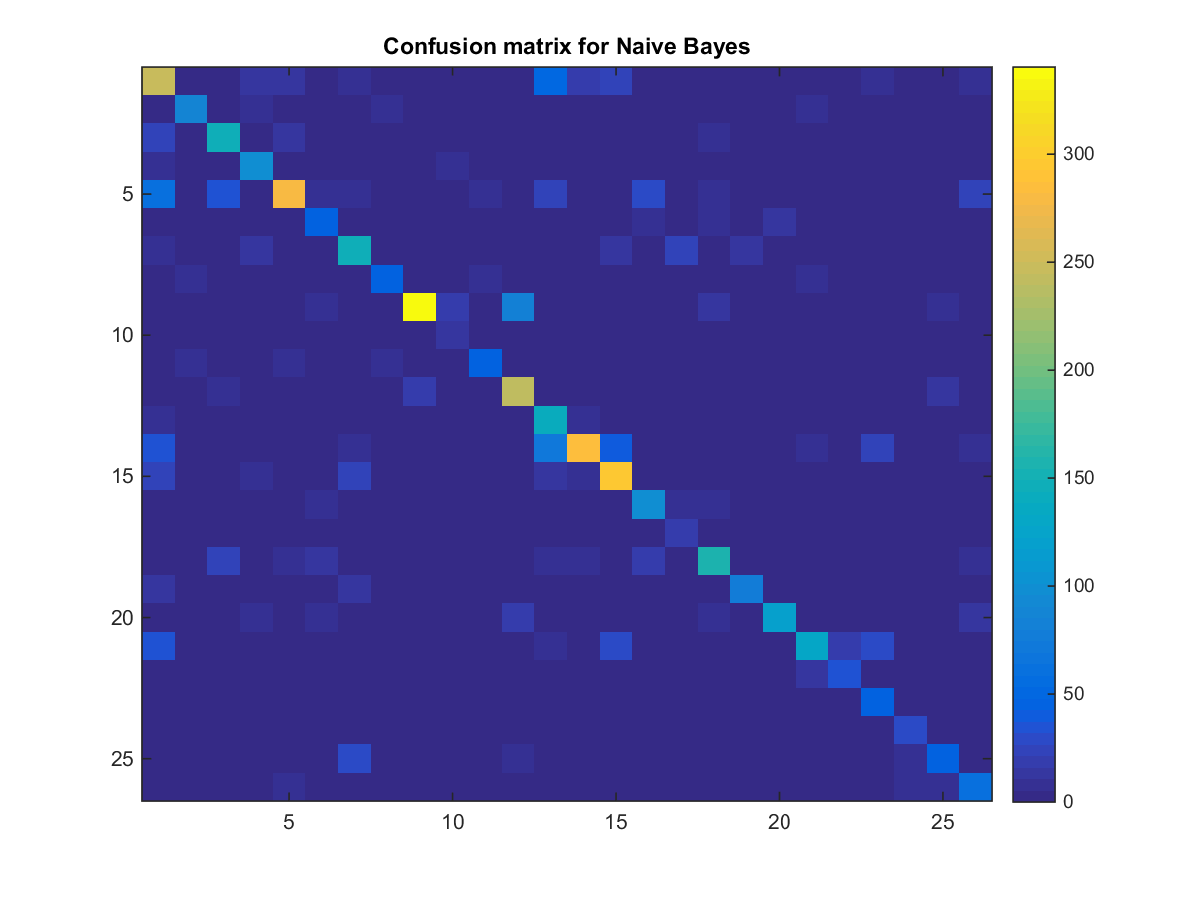
\includegraphics[scale=0.3]{confusionnb.png}
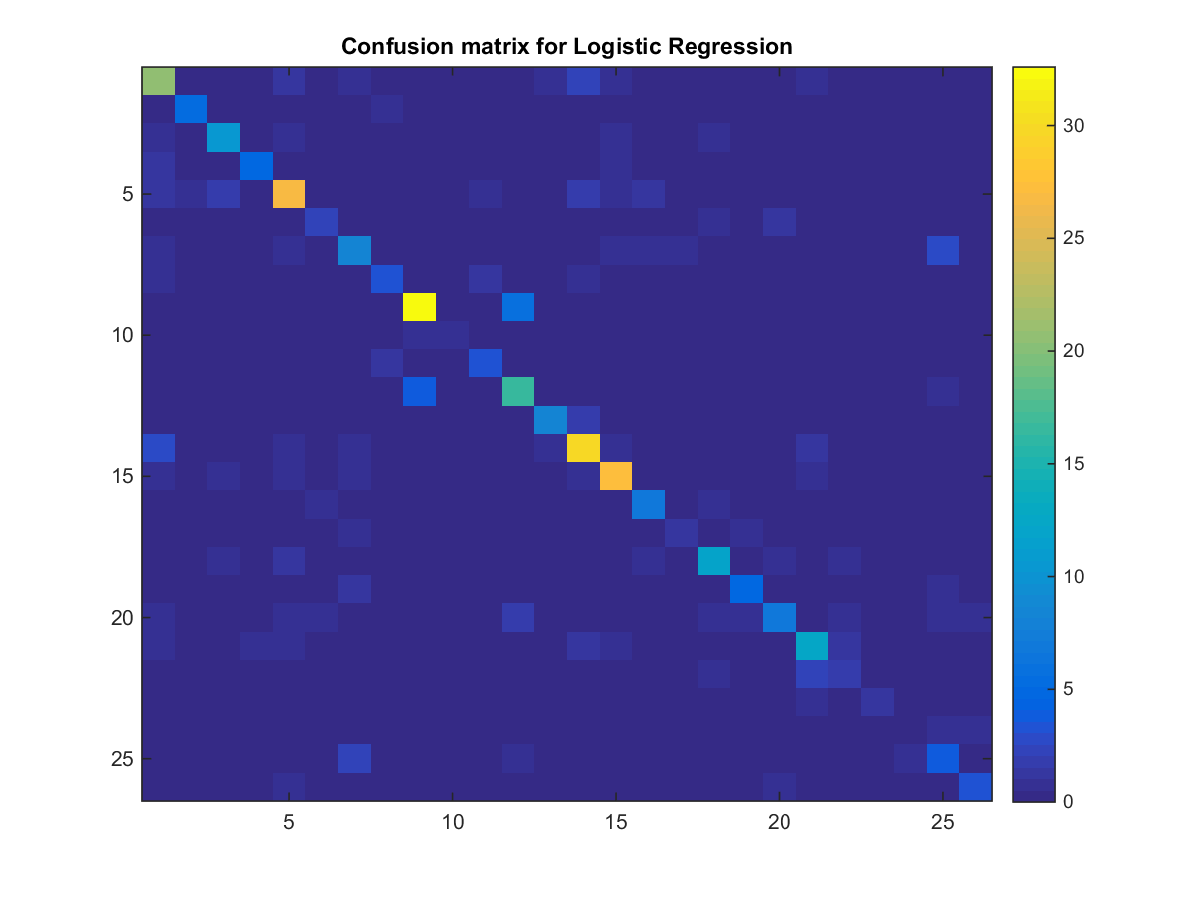
\includegraphics[scale=0.3]{confusionlr.png}
\end{center}
\caption{Visualization of the confusion mats for baseline classifiers}
\end{figure}

\subsection{Tables}

All tables must be centered, neat, clean and legible. Do not use hand-drawn
tables. The table number and title always appear before the table. See
Table~\ref{sample-table}.

Place one line space before the table title, one line space after the table
title, and one line space after the table. The table title must be lower case
(except for first word and proper nouns); tables are numbered consecutively.

\begin{table}[t]
\caption{Sample table title}
\label{sample-table}
\begin{center}
\begin{tabular}{ll}
\multicolumn{1}{c}{\bf PART}  &\multicolumn{1}{c}{\bf DESCRIPTION}
\\ \hline \\
Dendrite         &Input terminal \\
Axon             &Output terminal \\
Soma             &Cell body (contains cell nucleus) \\
\end{tabular}
\end{center}
\end{table}


\subsubsection*{Acknowledgments}

Use unnumbered third level headings for the acknowledgments. All
acknowledgments go at the end of the paper. Do not include 
acknowledgments in the anonymized submission, only in the 
final paper. 

\subsubsection*{References}

\small{
[1] Ivan Dervisevic(2006) {\it Machine Learning Methods for Optical Character Recognition.} \url{http://perun.pmf.uns.ac.rs/radovanovic/dmsem/complete/2006/OCR.pdf}

[2] Paolo Frasconi, Giovanna Soda, Alessandro Vullo (2001) {\it Text Categorization for Multi-page Documents: A Hybrid Naive Bayes HMM Approach.} \url{http://citeseerx.ist.psu.edu/viewdoc/download?doi=10.1.1.28.3940&rep=rep1&type=pdf}
}

\end{document}
